\documentclass{ncc}
\usepackage[utf8]{inputenc}
\usepackage[russian]{babel}
\usepackage[T2A]{fontenc}
\usepackage{amssymb}
\usepackage{amsmath}
\usepackage{pscyr}
\usepackage{graphicx}
\usepackage{listings}
\usepackage[colorlinks,linkcolor=black,urlcolor=blue]{hyperref}

\lstloadlanguages{C++}
\lstset{
language=C++,
extendedchars=\true, %Чтобы русские буквы в комментариях были
keepspaces=true,
inputencoding=utf8,
breaklines,
columns=fullflexible,
flexiblecolumns,
numbers=left,
numberstyle={\footnotesize},
commentstyle=\it,
stringstyle=\bf,
belowcaptionskip=5pt }


\title{Решение уравнений на комплексной плоскости}

\begin{document}
\maketitle
\tableofcontents
На прошлой неделе мы с \href{https://github.com/sputnikas}{Сергеем} столкнулись с новой для нас задачей, о которой ранее
не задумывались: потребовалось найти все комплексные корни уравнения \( f(z) =
0 \). В связи с новизной этой проблемы мы начали перебирать различные варианты
решения, в основном неудачные.


\section{Подход первый: сведение к системе уравнений}

Функцию комплексного переменного можно рассматривать как пару функций двух
действительных переменных переменных и свести исходную задачу к системе
\[
    f(z) = 0 \Leftrightarrow
    \begin{cases}
    u(x,y) = \mathrm{Re\,} f(x+iy) = 0,\
    v(x,y) = \mathrm{Im\,} f(x+iy) = 0,
    \end{cases}
\]
которую уже можно решать итерационными методами. Проблема заключается в том, что
мы хотим найти все корни этого уравнения (в некоторой конечной области,
разумеется). Итерационные методы же дают ответы в зависимости от начальных
приближений. Поэтому этот способ нам не подходит.

\section{Подход второй: точки неаналитичности функции}

Одна из самых знаменитых формул ТФКП, формула Коши, имеет вид
\[
    f(z_0) = \frac{1}{2\pi i}\oint\limits_{C} \frac{f(z)}{z-z_0}\,dz,
\]
где \(f(z)\) аналитическая всюду внутри контура и точка \(z_0\) лежит внутри
контура.

Рассмотрим интеграл
\[
    I = \frac{1}{2\pi i}\oint\limits_{C} \frac{1}{f(z)}\,dz
\]

Начнём с простого. Пусть \( f(z) = z - z_0 \). Тогда, если  \( z_0 \) лежит внутри контура, то \(I = 1\), а в противном случае \(I=0\).

Пойдём дальше и рассмотрим \(f(z) = (z-z_1)(z-z_2)\). Если контур охватывает сразу 2 корня то имеем
\[
I = \frac{1}{z_1 - z_2} + \frac{1}{z_2 - z_1} = 0.
\]
Уже не так хорошо.

Попробуем заменить 1  в числителе на некоторую функцию, например, рассмотрим
\[
    I = \frac{1}{2\pi i}\oint\limits_{C} \frac{f^\prime(z)}{f(z)}\,dz =
    \frac{1}{2\pi i}\oint\limits_{C}\, d \mathrm{Ln\,} f(z)
\]

Так как \( \mathrm{Ln\,} z = \ln |z| + i\mathrm{Arg\,} z \), то мы можем рассматривать изменения аргумента вдоль контура вместо интегрирования:
\[
    I = \frac{1}{2\pi}\oint\limits_{C}\, d \mathrm{Arg\,} f(z) = \frac{\Delta\mathrm{Arg\,}f(z)}{2\pi}.
\]
Это удобнее для программирования, так как вблизи корня для нахождения подынтегрального выражения придётся делить на очень маленькие числа, что может приводить к ошибкам.

\section{Подход третий: изменение аргумента}

Представим контур, который окружает область в которой мы ищем корень, в виде
параметрически заданной кривой \( z(t) \), причём \( z(0) = z(1) \).

Пусть точка \( 0 \) находится внутри контура. Определим непрерывную функцию
\[
    \phi(t) = \mathrm{Arg\,} z(t) - \mathrm{Arg\,} z(0),
\]
где значение аргумента выбирается в соответствии с условием непрерывности.
\begin{figure}[h]
\center
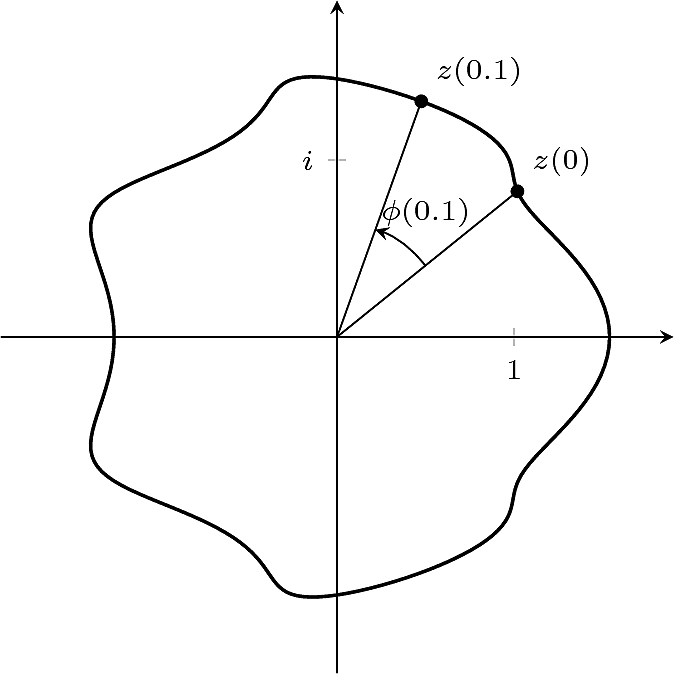
\includegraphics[width=.5\textwidth]{2015-10-26-complex-roots-contour.png}
\end{figure}
Введём также понятие изменение аргумента вдоль контура
\[
    \Delta \phi = \phi(1) - \phi(0) = \phi(1).
\]
Так как \(0\) находится внутри контура, то \( \Delta\phi = 2\pi \).

Будем говорить, что контур \( k \) раз оборачивается вокруг \(0\), если
\( \Delta\phi = 2\pi k \). Аналогично, контур \( k \) раз оборачивается
вокруг \( z_0 \), если \( z(t) - z_0 \) \(k\) раз оборачивается вокруг 0.
\begin{figure}[h]
\center
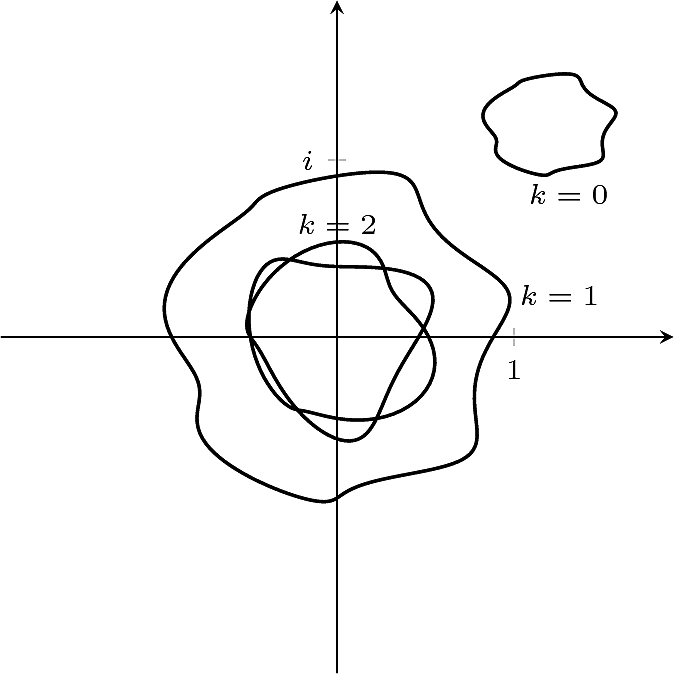
\includegraphics[width=.5\textwidth]{2015-10-26-complex-roots-rotations.png}
\end{figure}

Рассмотрим теперь контур вида
\[ z(t) = z_1(t)\cdot z_2(t). \]
Так как
\( \mathrm{Arg\,} z(t) = \mathrm{Arg\,} z_1(t) + \mathrm{Arg\,} z_2(t), \)
то \( \Delta \phi = \Delta \phi_1 + \Delta \phi_2 \), откуда для числа
оборотов контура имеем
\[ k = k_1 + k_2. \]

Пусть функция \( f(z) = (z-z_1)(z-z_2)(z-z_3)\cdots(z-z_n) \) некоторый
многочлен степени \( n \). Контур \(z(t)\) перейдёт в контур \(w(t) =
f(z(t))\), причём из вышесказанного следует, что число оборотов \( w(t) \)
вокруг нуля равно числу корней, оказавшихся внутри контура \( z(t) \).

Так как все многочлены над комплексным полем можно представить в виде
произведения линейных двучленов, то для любого многочлена число оборотов образа
контура вокруг \(0\) равно числу корней, если кратные корни считать различными.

Этот способ работает и для функций, представимых в виде ряда Тейлора всюду
внутри контура. В этот класс функций входят тригонометрические и гиперболические
функции, а также оговоренные выше многочлены. Доказать это можно, воспользовавшись интегралом, к которому мы пришли в предыдущей части:
\[
    I = \frac{1}{2\pi i}\oint\limits_{C} \frac{f^\prime(z)}{f(z)}\,dz = \frac{\Delta \phi}{2\pi}.
\]
Чтобы не усложнять доказательство, будем считать, что кратных корней у функции нет. Тогда используя формулу Коши, получим
\[
  I = \sum\limits_{i=1}^k \lim_{z\to z_i} \frac{f^\prime(z)(z-z_i)}{f(z)}
\]
Для функций, представимых в виде ряда Тейлора везде внутри области получим
\[
  f(z) = f(z_i) + f^\prime(z_i)(z-z_i) + o(z-z_i) = f^\prime(z_i)(z-z_i) + o(z-z_i).
\]
\[
  I = \sum\limits_{i=1}^k \lim_{z\to z_i} \frac{f^\prime(z)(z-z_i)}{f^\prime(z_i)(z-z_i)+o(z-z_i)}= \sum\limits_{i=1}^k 1 = k.
\]
Следовательно, число корней
\[
  k = \frac{\Delta\phi}{2\pi}.
\]

Теперь перейдём к более сложным функциям. Пусть \( f(z) = \sqrt{z} \). Это
двузначная функция, поэтому потребуем непрерывности отображения, какая бы ветвь
не была выбрана. Тогда \( z(t) = w(t)\cdot w(t) \). Отсюда, если корень внутри
контура, то \( \Delta\phi_w = \Delta\phi_z / 2 = \pi \), \( k = 1/2 \). В
противном случае так же получается \(0\). Обобщая, получаем, что для \( f(z) =
z^\alpha \) имеем \( k = \alpha \) если корень внутри контура.

Рассмотрим, наконец, отображение
\[
    f(z) = \frac{z+1}{z}.
\]
Если мы выберем в качестве контура окружность с центром в \(0\) и радиусом,
меньшим \(1\), то \(k = -1\). Если же взять такую же окружность с центром
в \(-1\), то \(k = 1\). Если же контур охватывает обе этих точки, то
\(k = 0\). Поэтому если присутствуют отрицательные степени нулевое изменение
аргумента не гарантирует отсутствия корней в области. Способ обойти это
ограничение очевиден -- привести всё выражение к общему знаменателю и
рассматривать только числитель.

\section{Алгоритм}
Для удобства деления пополам, в качестве области, в которой будем искать корни, удобно выбрать прямоугольник. Алгоритм похож на поиск в ширину на графе:

\begin{enumerate}
    \item Если внутри области есть корни, то положим исходный прямоугольник в очередь
    \item Пока очередь не пуста и диагональ прямоугольника больше погрешности определения корня:
    \begin{enumerate}
        \item Возьмем прямоугольник из очереди
        \item Разобъём его пополам вдоль длинной стороны
        \item Для получившихся прямоугольников определим число корней внутри
        \item Если корни внутри прямоугольников есть, то добавим их в очередь
    \end{enumerate}
    \item Центры оставшихся в очереди прямоугольников и есть искомые корни
\end{enumerate}

\begin{lstlisting}
cmplxs roots(func f, cmplx z1, cmplx z2, double eps) {
    std::queue<rectangle> rects;

    // небольшие сдвиги начальных границ, чтобы корни
    // с меньшей вероятностью легли на границу областей
    rectangle r = {z1 - eps, z2 + eps * cmplx(0, 1)};

    auto n = numberOfRoots(f, r);
    if (n == 0)
        return {};

    rects.push(r);
    while (!rects.empty() && rects.front().diag() > eps) {
        r = rects.front();
        rects.pop();

        rectangle r1, r2;
        r.divide(r1, r2);

        auto n1 = numberOfRoots(f, r1);
        auto n2 = numberOfRoots(f, r2);

        if (n1) rects.push(r1);
        if (n2) rects.push(r2);
    }

    cmplxs roots;
    while (!rects.empty()) {
        auto z = rects.front().center();

        if (std::abs(z.real()) < eps)
            z = cmplx(0, z.imag());
        if (std::abs(z.imag()) < eps)
            z = cmplx(z.real(), 0);

        roots.push_back(z);
        rects.pop();
    }

    return roots;
}
\end{lstlisting}

Для определения числа корней внутри прямоугольника используется функция
\begin{lstlisting}
unsigned int numberOfRoots(func f, cmplx z1, cmplx z2) {
    int n = 100;
    double angle = 0;
    cmplx zs[] = {z1, cmplx(z2.real(), z1.imag()),
                  z2, cmplx(z1.real(), z2.imag()), z1};
    double arg = NAN;
    for (int j = 0; j < 4; ++j)
    for (int i = 0; i < n; ++i) {
        auto z = (zs[j] * double(n-i) + zs[j+1] * double(i)) / n;
        double arg1 = std::arg(f(z));
        if (isnan(arg)) {
            arg = arg1;
            continue;
        }
        // дополняем старый аргумент до непрерывности с новым
        if (arg1 - arg > M_PI)
            arg += 2.0 * M_PI;
        if (arg - arg1 > M_PI)
            arg -= 2.0 * M_PI;
        angle += arg1 - arg;
        arg = arg1;
    }

    return std::abs((int) round(angle / M_PI / 2));
}
\end{lstlisting}

Код можно посмотреть \href{https://github.com/VSTU-physics/complex-roots}{здесь}.
\end{document}
